% Drawing 8/02-1 -- folder 8, batch 02, archive page 29 (PDF page 30).
% Transcription: page au stylo à bille, occupée pour moitié par des croquis : une région notée $C^1$ contenant des feuilles $\Phi_m$, $\Phi_n$ enroulées, un petit ouvert $U \supset V$ envoyé par $\sigma$ vers $\mathbb{R}^m$ (avec $\mathbb{R}^n$ dessiné dedans) ; ailleurs « $C^0$ », « $\emptyset$ », « $C^{\infty}$ » (surchargé), « $m-n$ », « $n-1$ »
% Kind: sheet of sketches: region C^1 with wound leaves, chart sigma to R^m. Method 2 (schematic redraw from the facsimile). Status: partial.
% Notes: Upper half of the sheet (ballpoint and pencil), redrawn on tight crops. Left: the region C^1 (doubled pencil oval) containing the leaf drawn in ink as one curve going back and forth five times (the accordion of a wound leaf), with four faint pencil strokes alongside; Phi_m is written at the top left of the oval, Phi_n inside. The small circle (the open U, which bears no legible letter of its own; a mark inside it may be a U or a second v) with the point and the letter V, and the arrow sigma down to R^m: a pencil cone (apex, one side and three hatchings), R^n the heavy stroke from the apex to the right, with a faint pencil stroke going up from the apex next to the label R^n. Pencil hatchings at the left schematised (one curve, four crossing strokes). Right: C^0 ringed, the empty set, C^infinity overwritten (label only), the doubled lens crossed by two heavy strokes, the ink arc at the right edge and n-1 beside it, and the faint pencil links (C^1 to the lens, C^1 to a small loop, the lens down to the big oval). The ink oval round the formulas sigma(V) = sigma(U) cap R^n and A_0 = {...} and the two pencil ovals inside it are drawn; the formulas, V_i subset U_i and the line "1) Familles canoniques C^r" (whose ink frame is drawn, cut by the crop) are text of the transcription. Still differs: the pencil doublings of every oval are drawn once, the pencil leaves and hatchings are schematic. Redrawn 2026-11-09 (issue 128): to check again.
% Coordinates: 1 unit = 1 mm = 1/100 of the crop width (bbox in page fractions: [0.05, 0.04, 0.98, 0.45]).
% Redrawn by Claude (claude-opus-5-5), issue #73, 2026-11-09; not checked by a human; not compiled (no TeX in the session).
% Rights: reproduces part of the work -- behind RENDER_TRANSCRIPTS, never published by itself.
\documentclass[tikz,border=3pt]{standalone}
\usepackage{amsmath,amssymb}
\usetikzlibrary{patterns,arrows.meta}
\tikzset{pencil/.style={black!45}, struck/.style={black!35}, mark/.style={circle,draw,inner sep=1.3pt}, pt/.style={circle,fill,inner sep=0.9pt}, opt/.style={circle,draw,fill=white,inner sep=1.1pt}}
\begin{document}
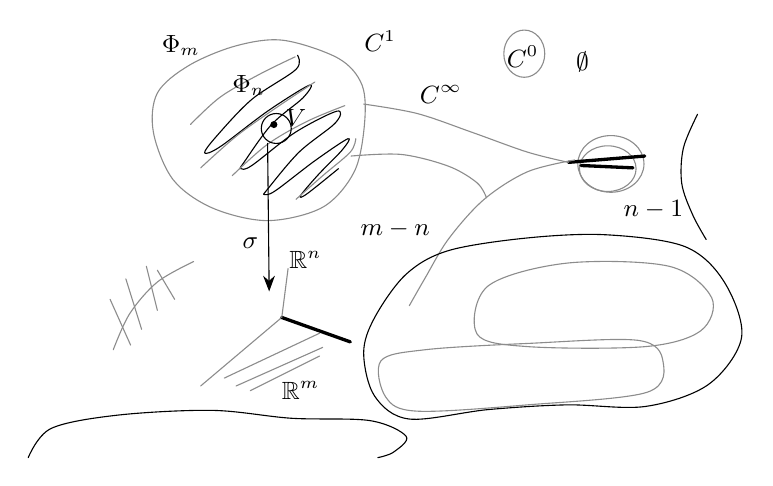
\begin{tikzpicture}[x=1mm,y=1mm,line cap=round,line join=round,font=\scriptsize]
\draw[pencil] plot[smooth cycle, tension=0.55] coordinates {(39,-9.3) (46,-11.6) (49,-15) (49.3,-20) (48,-26) (44,-30.5) (37,-32.2) (30,-30.6) (25,-27) (22.5,-21) (23,-16) (27,-12.5) (33,-10)};
\draw plot[smooth, tension=0.55] coordinates {(40.8,-11.2) (40.6,-13) (35,-16.8) (30.5,-21.5) (29,-23.6) (31,-22.8) (37,-18.3) (42.3,-15) (41.5,-16.6) (37.5,-20) (34,-24.8) (33.6,-25.6) (35,-25.2) (40.5,-21) (45.8,-18.3) (45.6,-19.8) (41,-23.5) (37,-28.2) (36.6,-28.9) (38,-28.4) (43,-24.6) (47.2,-21.8) (46.5,-23.2) (43.5,-26.3) (41.2,-29) (42,-28.8) (46,-25.6)};
\draw[pencil] plot[smooth, tension=0.55] coordinates {(27.2,-20) (31,-16.5) (36,-13.6) (40.5,-11.4)};
\draw[pencil] plot[smooth, tension=0.55] coordinates {(28.5,-25.5) (33,-21.5) (37.6,-18.2) (43,-14.6)};
\draw[pencil] plot[smooth, tension=0.55] coordinates {(32.5,-26.5) (37,-22.5) (42,-19.6) (46.8,-17.6)};
\draw[pencil] plot[smooth, tension=0.55] coordinates {(40.6,-29.5) (44,-26.5) (47.5,-23.5) (48.2,-21.8)};
\draw (38.1,-20.5) circle[radius=1.9];
\node[pt] at (37.8,-20) {};
\draw[-{Stealth[length=2mm]}] (37,-22.4) -- (37.2,-41.2);
\draw[pencil] (38.8,-44.5) -- (28.5,-53.2);
\draw[very thick] (38.8,-44.5) -- (47.5,-47.6);
\draw[pencil] (38.8,-44.5) -- (39.6,-38.3);
\draw[pencil] (31.5,-52.2) -- (43.6,-46.5);
\draw[pencil] (33,-53.2) -- (44,-48.3);
\draw[pencil] (34.8,-53.8) -- (43.6,-49.4);
\draw[pencil] plot[smooth, tension=0.55] coordinates {(17.4,-48.6) (19.5,-44) (23,-40) (27.6,-37.4)};
\draw[pencil] (17,-42.2) -- (19.6,-48);
\draw[pencil] (19,-39.6) -- (21,-46);
\draw[pencil] (21.6,-38) -- (23,-43.6);
\draw[pencil] (23,-38.5) -- (25.2,-42.2);
\draw[pencil] (69.6,-11) ellipse[x radius=2.6, y radius=3];
\draw[pencil] (80.6,-25) ellipse[x radius=4.2, y radius=3.6];
\draw[pencil] (80.2,-25.6) ellipse[x radius=3.6, y radius=2.9];
\draw[very thick] (75.2,-24.8) -- (84.9,-24);
\draw[very thick] (76.8,-25.2) -- (83.4,-25.5);
\draw plot[smooth, tension=0.55] coordinates {(91.6,-18.7) (89.8,-23) (89.6,-27.5) (91,-31.5) (92.7,-34.6)};
\draw[pencil] plot[smooth, tension=0.55] coordinates {(49.2,-17.4) (56,-18.6) (63,-21) (70,-23.5) (75.2,-24.8)};
\draw[pencil] plot[smooth, tension=0.55] coordinates {(47.6,-24) (54,-23.8) (60,-25.3) (63.6,-27.4) (64.8,-29.3)};
\draw[pencil] plot[smooth, tension=0.55] coordinates {(76,-24.5) (70,-26) (64.5,-29.5) (60,-34.5) (57,-39.5) (55,-43)};
\draw plot[smooth cycle, tension=0.55] coordinates {(60,-36) (70,-34.4) (80,-34) (90,-35.5) (95,-40) (97.2,-47) (93,-53) (85,-55.8) (75,-55.6) (65,-56.2) (55,-57.4) (50.6,-54.5) (49.2,-49) (50.6,-44.5) (54.6,-39)};
\draw[pencil] plot[smooth cycle, tension=0.55] coordinates {(63.6,-46.6) (65,-40.5) (75,-37.6) (88,-38) (93.4,-42) (92,-46.2) (85,-48.2) (70,-48.2)};
\draw[pencil] plot[smooth cycle, tension=0.55] coordinates {(52,-54.6) (51.4,-50) (57,-48.6) (70,-47.8) (84,-47.4) (87.2,-50) (85.2,-54) (70,-55.6) (56,-56.4)};
\draw plot[smooth, tension=0.55] coordinates {(6.6,-62.3) (9.5,-58.6) (18,-56.9) (30,-56.3) (40,-57.3) (50,-57.6) (54.6,-59.6) (53,-61.6) (51,-62.3)};
\node[inner sep=1pt] at (26,-10) {\small $\Phi_m$};
\node[inner sep=1pt] at (34.6,-15) {\small $\Phi_n$};
\node[inner sep=1pt] at (51.3,-9.4) {\small $C^1$};
\node[inner sep=1pt] at (40.6,-19.2) {\small $V$};
\node[inner sep=1pt] at (34.8,-35) {\small $\sigma$};
\node[inner sep=1pt] at (41.8,-37.2) {\small $\mathbb{R}^n$};
\node[inner sep=1pt] at (41.2,-53.8) {\small $\mathbb{R}^m$};
\node[inner sep=1pt] at (53.2,-33.3) {\small $m-n$};
\node[inner sep=1pt] at (59,-16.2) {\small $C^{\infty}$};
\node[inner sep=1pt] at (69.4,-11.4) {\small $C^0$};
\node[inner sep=1pt] at (77,-12) {\small $\emptyset$};
\node[inner sep=1pt] at (86,-30.8) {\small $n-1$};
\end{tikzpicture}
\end{document}
